\chapter{\label{ch:ch5} Design Case Study}

\section{Design Specifications \label{sec:design-specs}}

The methodology and design considerations described in the previous chapter were implemented in a case study design as reported in following chapter. The chapter begins with a description of the specifications of each subsystem and follows with the acceptance test procedures (ATPs) for each subsystem before concluding with the integration test procedures. The first section specifies the hardware components and operation of the SPQIS which involves the 32-bit microntroller and a set of timing constraints for modelling the decoherence times of the initialised qubits. Normalised qubit probabilites were generated in MATLAB and preloaded to the devices to ensure that the probabilistic nature of quantum computers is maintained. 

The FQDS specifications include details about the electronic circuit used to model the quantum channel. The parameters of particular interest include the input and output voltages, current, resistances as well as the physical layout of the design. Since the electronic circuit also includes a NPN-type BJT, other paramaters such as base, collector and emitter voltages and currents are included to characterise the FQDS. 

High-level descriptions of quantum algorithms in MATLAB are specified in the QAES specifications section. This sections also shows snippets of SystemVerilog code used to simulate the RTL behaviour of the system. Further information is provided on the AMD Vivado IP Cores and other resources utilised during the emulation of the quantum algorithms on the Nexys A7 FPGA. The quantum algorithms explored in the design case study included the quantum teleportation algorithm for transferring quantum state information through a quantum channel, the QFT for changing between the computational basis and the Fourier basis, as well as the quantum factoring and quantum search algorithms. Specifically, the case study for emulating the quantum factoring algorithm involved finding the order $r$ of $N = 21$ with an initial guess of $x = 4$, using the quantum circuit in \ref{fig:quantum-factoring-algorithm}. Depending on the quantum circuit and the algorithm performed, quantum gate operations were implemented as FSM or as matrix multiplication operations. 

Specifications of the UIS detail steps for operating each subsystem. In line with quantum mechanical constraints on observations of quantum states, users can prepare initial qubit states and measure the quantum circuit outputs but do not have access to intermediate results from quantum gate operations. Hence, the section on the UIS specification includes instructions for initialising qubits on the microcontroller, selection of the desired quantum circuit emulation experiment, and the manner in which outputs are displayed to the user. 

\subsection{Single-Photon Qubit Initialisation Subsystem Specifications \label{subsec:sqpis-specs}}

\subsubsection{Generate a Normalised Distribution of Probabilities $n$-Qubit Systems}

To maintain the probabilistic nature of quantum computers across the simulation, pure quantum state probabilities were generated using the MATLAB \texttt{randn} function to return normally distributed random numbers as seen in listing \ref{lst:normally-distributed-probabilities} showing a code snippet of the \texttt{generate\_probs} function. In this study of the proposed design, the first qubit in the $n$-qubit quantum register $\ket{q_0 q_1 ... q_{n-1}}$ is the MSB and the last qubit $\ket{q_{n-1}}$ in the register is taken as the LSB. 

\begin{lstlisting}[language=Matlab, caption={MATLAB script for generating pseudo random numbers for the probabilities associated with quantum states.}, label={lst:normally-distributed-probabilities}]
	function amplitude_squared = generate_probs(n)
	
	% The total number of possible states for n qubits is 2^n
	num_states = 2^n;
	
	% Generate the random values using the pseudorandom generator
	random_values = randn(1, num_states);
	
	% Take the absolute values to ensure non-negative probabilities
	abs_values = abs(random_values);
	
	% Normalise the values to make them valid probabilities (sum to 1)
	amplitude_squared = abs_values / sum(abs_values);
	
	% Display the probabilities
	disp('Generated Quantum State Probabilities:');
	disp(amplitude_squared);
	end
\end{lstlisting}

The \texttt{generate\_probs} function takes in the number of qubits $n$ to create $2^n$ probabilities. Since probabilities are the normalised magnitudes of pure (real) quantum states, the built-in \texttt{abs} is used to ensure that the generated probabilities are positive. The table indicates the number of qubits that are initialised for each quantum algorithm and the generated probabilities. Since most qubit registers are initialised in the ground state, the outputs of the \texttt{generate\_probs} function that are valid for this application are such that the probability of measuring the ground state is the greatest. 

Selection of the probabilities introduces deterministic effects in the model which is not ideal for this case study. Therefore, the acceptance test for \texttt{generate\_probs} function needs to verify that the pseudo-random selection process generates normalised values. The output of the \texttt{generate\_probs} is transferred to the STM32 microcontroller and the Nexys A7 FPGA in the FQDS subsystem. 

\subsubsection{Initialise Qubits on the STM32 Microcontroller Using Push-Buttons}

The UCT STM32F0 Development Board employed in the case study is an entry-level 32-bit ARM microcontroller unit which incorporates the Corext-M0 processor designed for a variety of embedded systems applications. Specifically, the  STM32F0 board contains a Cortex-M0 processor which implements a 3-stage pipeline ARMv6-M von Neumann architecture with internal memory. The microcontroller is powered through a standard USB connection which provides a 5V regulated supply of up to 500 mA. When power is supplied to the board, a green LED on the board turns on to indicate to the user that the board is operational. Table \ref{tab:microcontroller-power} shows further hardware specifications for ensuring that the device is operating correctly. 
\begin{table}[ht!]
	\centering
	\caption[Table Showing the Hardware Specifications of the STM32F0 Microcontroller Used to Initialise Qubits and Control Flying-Qubit Emissions.]{Table showing the hardware specifications of the STM32F0 microcontroller used to initialise qubits and control flying-qubit transmissions.}
	\label{tab:microcontroller-power}
	\setlength\tabcolsep{0pt} % let LaTeX compute intercolumn whitespace
	\footnotesize\centering
	\begin{tabular*}{\columnwidth}{@{\extracolsep{\fill}}|c|l|l|}
		\hline
		\textbf{Callout} & \textbf{Description} & \textbf{Value}\\
		\hline
		1		& Input Power & $\SI{5.0}{\volt}$;$\SI{500}{\milli\ampere}$\\
		\hline
		2		& Operating Voltage  & $\SI{2.0}{\volt}$ to $\SI{3.6}{\volt}$\\
		\hline
		3		& Maximum Clock Frequency  &	$\SI{48}{\mega\hertz}$  \\
		\hline
		4		& Operating Temperature	   &	$-\SI{40}{\degreeCelsius}$ to $\SI{85}{\degreeCelsius}$\\
		\hline
	\end{tabular*}
\end{table}

The processor is connected to multiple external peripherals and circuits. An ST-LINK/V2 in-circuit debugger connects to the STM32F051C6 daughter board though the serial wire debug interface that allows code to be compiled, uploaded and stepped through to fix runtime errors. In this case study, quantum state probabilities produced by the \texttt{generate\_probs} MATLAB script are written in a C header file (\textit{quantum\_state.h}) and uploaded to flash memory through the serial wire debug interface as shown in the code snippet in listing \ref{lst:upload-probabilities}. In particular, the snippet shows the initialisation of qubits to the ground state whereby the real amplitude of the $\ket{0}^{\otimes n}$ state is set to 1, corresponding to a normalised probability of 1. 
\begin{lstlisting}[language=C, caption={Snippet code from C header file for initialising qubits in the STM32 microcontroller.}, label={lst:upload-probabilities}]
	// Define a complex number structure to represent quantum amplitudes
	typedef struct {
		float real;    // Real part of the amplitude
		float imag;    // Imaginary part of the amplitude
	} complex_t;
	
	//====================================================================
	// GLOBAL VARIABLES FOR QUANTUM STATES
	//--------------------------------------------------------------------
	
	// 1-qubit quantum register (2 possible states: 
	//|0> and |1>)
	complex_t quantum_state_1q[2] = {
		{1.0, 0.0},  // Amplitude of |0> state
		{0.0, 0.0}   // Amplitude of |1> state
	};
	
	// 2-qubit quantum register (4 possible states: 
	//|00>, |01>, |10>, |11>)
	complex_t quantum_state_2q[4] = {
		{1.0, 0.0},  // Amplitude of |00> state
		{0.0, 0.0},  // Amplitude of |01> state
		{0.0, 0.0},  // Amplitude of |10> state
		{0.0, 0.0}   // Amplitude of |11> state
	};

	// ... remove code blocks for up to 5-qubits
	
	void initQuantumState(complex_t* state, uint8_t num_states);
\end{lstlisting}
The code in \ref{lst:upload-probabilities} hosts a function, named \texttt{initQuantumState} for initialising the qubits to a fiduciary state depending on the selected quantum algorithm. Since the quantum algorithms performed require up to 5-qubits, the \texttt{initQuantumState} function can initialise qubit registers with up to $n = 5$ qubits. If a quantum algorithm is not selected or the board is reset, then the system automatically initialises the two-qubit register $\ket{00}$. Note that on the microcontroller, qubit initialisations represent the set of the monochromatic laser for transmitting single-photon qubits through the quantum channel in the FQDS subsystem. 

In addition to initialising fiduciary state, the SPQIS allows users to prepare entangled qubits for performing the quantum teleportation algorithm as shown in code listing \ref{lst:prepare-entangled-state}.

\begin{lstlisting}[language=C, caption={Further code from the \textit{quantum\_state.h} C header file for peparing EPR pairs.}, label={lst:prepare-entangled-state}]
	// ... removed code block
	
	// Function to prepare an entangled quantum state pair (Bell state)
	void prepareEntangledPair(complex_t* state);
	
	// Prepare an entangled quantum state pair 
	// (Bell state |+> = (|00> + |11>) / sqrt{2})
	void prepareEntangledPair(complex_t* state) {
		float norm = 1.0 / sqrt(2);  // Normalisation factor (1/sqrt{2})
		
		// Set the amplitudes for the Bell state
		// |+> = (|00> + |11>) / sqrt{2}
		state[0].real = norm;  // Amplitude of |00>
		state[0].imag = 0.0;
		
		state[3].real = norm;  // Amplitude of |11>
		state[3].imag = 0.0;
		
		// Set other states' amplitudes to 0 (|01> and |10>)
		state[1].real = 0.0;   // Amplitude of |01>
		state[1].imag = 0.0;
		
		state[2].real = 0.0;   // Amplitude of |10>
		state[2].imag = 0.0;
	}
	#endif /* QUANTUM_STATE_H */
\end{lstlisting}
This \texttt{prepareEntangledPair} function is used during emulation of the quantum teleportation algorithm in which prior entanglement information is shared between Alice and Bob. When the microcontroller is reset or restarted, qubits return to the separable ground state. 
 
\subsection{Flying-Qubit Detection Subsystem Specifications \label{subsec:fqds-specs}}

The pins of the microcontroller are illustrated in figure \ref{fig:stm32-pins}. The design case study uses these pins to model the quantum interface which facilitates quantum and classical communication between the microcontroller and the quantum computer emulated on the FPGA. 
\begin{figure}[!ht]
	\centering
	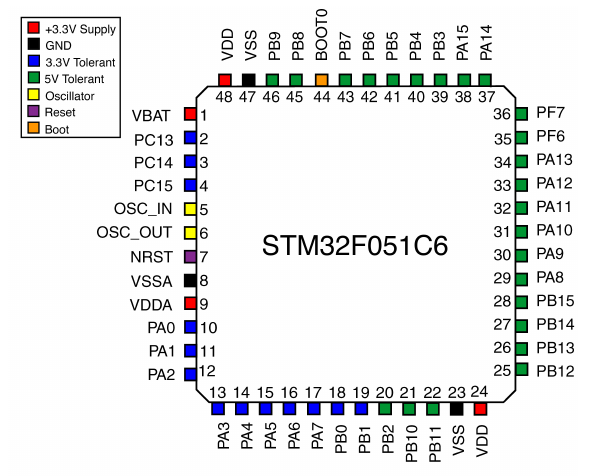
\includegraphics[width=0.90\linewidth]{body/ch5/figs/stm32f051c6}
	\caption[Showing Input and Output Pins on the STM32 Microcontroller.]{The input and output pins on the microcontroller are implemented in the model of the quantum interface which consists of a quantum channel and classical channel.}
	\label{fig:stm32-pins}
\end{figure}
The system uses 8 LEDs to model monochromatic lasers pulses. The LEDs are connected to the microcontroller through GPIO port B as shown in the table \ref{tab:led-connections}. 
\begin{table}[ht!]
	\caption[Table Showing LED Connections to the STM32 Microcontroller.]{Table showing the fixed relationship between laser-modelling LEDs and GPIO port B pins of the microcontroller.}
	\label{tab:led-connections}
	\setlength\tabcolsep{0pt} % let LaTeX compute intercolumn whitespace
	\footnotesize\centering
	\begin{tabular*}{0.45\columnwidth}{@{\extracolsep{\fill}}|c|c|}
		\hline
		\textbf{LED Label} & \textbf{GPIO Pin~~~~~~~~~}\\
		\hline
		L0		& PB7 \\
		\hline
		L1		& PB6 \\
		\hline
		L2		& PB5 \\
		\hline
		L3		& PB4	 \\
		\hline
		L4		& PB3 \\
		\hline
		L5		& PB2	 \\
		\hline
		L6		& PB1	 \\
		\hline
		L7		& PB0	 \\
		\hline
	\end{tabular*}
\end{table}

The function called \texttt{initGPIO}, as seen in listing \ref{lst:init-port-b}, is used to enable the clock and mode registers for port B as an output for modelling transmissions of single-qubit quantum states. Note that port A is enabled as an input so that buttons can be used to initialise the required ground states for each quantum algorithm. 
\begin{lstlisting}[language=C, caption={Showing the \texttt{initGPIO} function for enabling ports B as a outputs and ports A as inputs.}, label={lst:init-port-b}]
void initGPIO() {
	uint32_t *RCCADDR = (uint32_t*)(0x40021000 + 0x14);
	
	*RCCADDR |= 0b1 << 18;  // Enable clock for port B
	*RCCADDR |= 0b1 << 17;  // Enable clock for port A
	
	// Enable mode register for port B as output (for LEDs)
	GPIOB->MODER |= GPIO_MODER_MODER0_0;
	GPIOB->MODER |= GPIO_MODER_MODER1_0;
	GPIOB->MODER |= GPIO_MODER_MODER2_0;
	GPIOB->MODER |= GPIO_MODER_MODER3_0;
	GPIOB->MODER |= GPIO_MODER_MODER4_0;
	GPIOB->MODER |= GPIO_MODER_MODER5_0;
	GPIOB->MODER |= GPIO_MODER_MODER6_0;
	GPIOB->MODER |= GPIO_MODER_MODER7_0;
	
	// Set mode register for port A as input (for switches)
	GPIOA->MODER &= ~GPIO_MODER_MODER0_0;
	GPIOA->MODER &= ~GPIO_MODER_MODER1_0;
	GPIOA->MODER &= ~GPIO_MODER_MODER2_0;
	GPIOA->MODER &= ~GPIO_MODER_MODER3_0;
	
	// Enable pull-up resistors for switches
	GPIOA->PUPDR |= GPIO_PUPDR_PUPDR0_0;
	GPIOA->PUPDR |= GPIO_PUPDR_PUPDR1_0;
	GPIOA->PUPDR |= GPIO_PUPDR_PUPDR2_0;
	GPIOA->PUPDR |= GPIO_PUPDR_PUPDR3_0;
}
\end{lstlisting}

\subsubsection{Transmit Qubits in the Quantum Channel of the Quantum Interface}

Table \ref{tab:led-connections} indicates that using the first mode of transmission, the system can transmit quantum registers with up to 8 qubits in total. To model qubit registers in the computational basis, bit patterns are transferred to the 8-bit mode registers for GPIO port B as shown in table \ref{tab:mode-1-qubits}. The table shows the number of qubits in the register, the quantum state register with probability 1 that is to be transmitted, and the expected number of sequences $s_1$ to be transmitted. Base on table \ref{tab:led-connections}, it can be seen that the L0 is associated with the LSB and L7 is associated with the MSB. Therefore, bit patterns need to be reversed in order to transfer qubits accurately through the system. The pattern column in \ref{tab:mode-1-qubits} shows the decimal conversion of the reversed bit pattern.
\begin{table}[ht!]
	\caption[Table Showing the Transmitted Flying-Qubit Registers Using Transmission Mode 1.]{Table showing the number $n$ of qubits in the register, qubits in the register, transmitted bit pattern as a decimal number, and the expected number of sequences $s_1$.}
	\label{tab:mode-1-qubits}
	\setlength\tabcolsep{0pt} % let LaTeX compute intercolumn whitespace
	\footnotesize\centering
	\begin{tabular*}{0.8\columnwidth}{@{\extracolsep{\fill}}|c|c|l|l|}
		\hline
		\textbf{n} & \textbf{Quantum Register~~~~~} & \textbf{Pattern} & $\mathbf{s}_1$\\
		\hline
		4		& $\ket{10}_{10}$ &  $5_{10}$ & 1\\
		\hline
		8		& $\ket{43}_{10}$ & $212_{10}$ & 1\\
		\hline
		16		& $\ket{233}_{10}$ & $151_{10}$ & 2\\
		\hline
		32		& $\ket{21713}_{10}$ & $17813_{10}$ & 4\\
		\hline
	\end{tabular*}
\end{table}
Qubit decoherence times are modelled using a $\SI{340}{\milli\second}$ delay in the C code for toggling full bit sequences. The decoherence time of qubits is critical for setting the detection window on the emulated quantum computer.

A similar table is used to transmit the Hilbert spaces of qubits through the quantum channel as shown in \ref{tab:mode-2-qubits}. The expected number of sequences required to transmit a full qubit register with $n$ qubits is also shown. However, when transferring Hilbert spaces, $2^n$ units of information are transferred by each LED. This implies that for $n = 32$, $2^{32}$ qubits are required to fully represent the quantum state. However, only one LED switches on during the entirety of the process, correspond the index of 1 in the Hilbert space of the qubit.
\begin{table}[ht!]
	\caption[Table Showing the Transmitted Flying-Qubit Registers Using Transmission Mode 2.]{Table showing the number $n$ of qubits in the register, qubits in the register, transmitted bit pattern as a decimal number, and the expected number of sequences $s_2$.}
	\label{tab:mode-2-qubits}
	\setlength\tabcolsep{0pt} % let LaTeX compute intercolumn whitespace
	\footnotesize\centering
	\begin{tabular*}{0.87\columnwidth}{@{\extracolsep{\fill}}|c|c|l|l|}
		\hline
		\textbf{n} & \textbf{Quantum Register~~~~~} & \textbf{Pattern} & $\mathbf{s}_2$\\
		\hline
		4		& $\ket{10}_{10}$ &  $1024_{10}$ & 2\\
		\hline
		8		& $\ket{43}_{10}$ & $2097152_{10}$ & 32\\
		\hline
		16		& $\ket{233}_{10}$ & - & -\\
		\hline
		32		& $\ket{21713}_{10}$ & - & -\\
		\hline
	\end{tabular*}
\end{table}
The two methods are compared to infer on the communication complexity of the quantum channel. The second method was expected to have a larger communication complex than the first method due to the large amount of information that needs to be transferred. The communication complex was measured by the number of sequences and times required to transmit on qubit register.

\subsubsection{Flying-Qubit Detection System}

Flying qubits are transmitted through a model of the fibre link in QKD networks using cut paper straws. Paper straws were chosen as a security measure to prevent eavesdropping on the quantum channel. A diagram of a single detection circuit is illustrated in figure \ref{fig:fqds-circuit} with values as shown in table \ref{tab:fqds-values}. In the case study, the circuit shown is duplicated eight times and connected to the Pmod I/O pins of the FPGA. To model the conversion of qubits in the computational basis, the LDR and $R_1$ are used to divide the voltage such that when the LDR is occluded (inactive), the base voltage of the transistor Q approaches zero and when light from the LED is incident on the LDR (active), the base voltage exceeds the base-emitter voltage of $\SI{1.4}{\volt}$. Once the base voltage exceeds the base-emitter voltage, the transistor becomes saturated, allowing current to flow through the collector. The collector resistor $R_C$ was implemented to ensure that the current is well below the maximum $\SI{24}{\milli\ampere}$ of the FPGA input ports.
\begin{figure}[!ht]
	\centering
	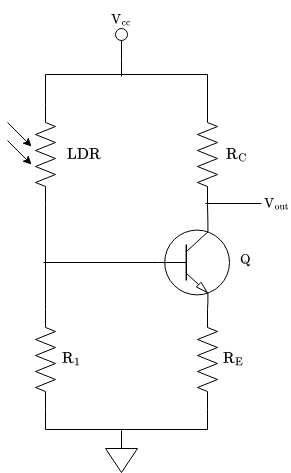
\includegraphics[width=0.45\linewidth]{body/ch5/figs/fqds-circuit}
	\caption[Simple Circuit Diagram for Modelling Avalanche Photodiode Detectors in a QKD network.]{The circuit shown is used to in the case study to model APDs. Corresponding values can be found in \ref{tab:fqds-values}}
	\label{fig:fqds-circuit}
\end{figure}

\begin{table}[ht!]
	\caption[Table Showing Circuit Component Values for the Quantum Interface.]{Specifications of the electronic circuit for modelling the quantum channel.}
	\label{tab:fqds-values}
	\setlength\tabcolsep{0pt} % let LaTeX compute intercolumn whitespace
	\footnotesize\centering
	\begin{tabular*}{0.50\columnwidth}{@{\extracolsep{\fill}}|c|c|}
		\hline
		\textbf{Label} & \textbf{Value} \\
		\hline
		$V_{CC}$		& $\SI{3.3}{\volt}$ \\
		\hline
		$LDR$	(inactive)	& $\SI{1}{\mega\ohm}$ \\
		\hline
		$LDR$	(active)	& $\SI{400}{\ohm}$ \\
		\hline
		$R_E$		& $\SI{220}{\ohm}$ \\
		\hline
		$R_C$		& $\SI{1}{\kilo\ohm}$ \\
		\hline
	\end{tabular*}
\end{table}

As mentioned, the aim of the circuit is to model the conversion of flying-qubits to stationary qubits while ensuring that the maximum current that the inputs of the FPGA can take is not exceeded.  The maximum current of the FPGA inputs is $\SI{24}{\milli\ampere}$. Using the values in \ref{tab:fqds-values}, the expected maximum current through the circuit was $\SI{3.3}{\milli\ampere}$. 

The design case study implements the electronic circuit iteratively, beginning with a prototype built on a bread, followed by a final version on breadboard or PCB. 

\subsection{Quantum Algorithm Subsystem Specifications \label{subsec:qaes-specs}}

\subsubsection{Universal Set of Quantum Gates}

To reduce development time, the design case uses MATLAB as high-level description of the quantum gate operations. Following the high-level description of algorithm involved in the unitary transformation of qubits, HDL Coder is used to generate SystemVerilog code and Simulink is used to simulate the signals involved in the system. Another benefit of using MATLAB and HDL Coder is that it can be setup to use Xilinx Vivado to run simulations, synthesis and the implementation of the system on the target board. 

Based on the algorithms applied in the design, the quantum gates that are described in MATLAB include the \texttt{X} gate, the \texttt{H} gate and the \texttt{CNOT} gate (or $\Lambda \texttt{X}$ gate). These gates were chosen in for the design case because they represent the basic operations in the set of universal quantum gates of the emulated quantum computer.

The emulated \texttt{X} gate is described simply as shown in the code snippet in listing \ref{lst:x-gate-matlab} below. To successfully implement HDL Coder in the design, the high-level description is written as a function \texttt{x\_gate} with an accompanying testbench script as shown in listing \ref{lst:x-matlab-testbench}. The \texttt{x\_gate} function takes in an input \textit(state) which is a 2x1 column vector representing the initial quantum state in the computational basis and rotates Hilbert space to an orthogonal basis. That is, if the input is $\ket{0}$, then the expected output is $\ket{1}$ as described in the previous sections. Although this can be applied using a simple FSM, the use of HDL Coder allows designs to be created using a few LUTs on the target FPGA.
\begin{lstlisting}[language=Matlab, caption={Code snippet of the MATLAB high-level description of the \texttt{X} gate applied to a single qubit in the state $\ket{0}$.}, label={lst:x-gate-matlab}]
function new_state = x_gate(state)
	% Apply the Pauli-X gate to a single qubit
	% state - a 2x1 column vector representing the
	% qubit state, e.g., [1; 0] for |0> or [0; 1] for |1>
	% Returns:
	% new_state - the resulting state 
	% after applying the X gate
	
	% Define the Pauli-X gate (NOT gate)
	X = [0, 1; 
	1, 0];
	
	% Apply the X gate to the input qubit state
	new_state = X * state;
end
\end{lstlisting}
The testbench of the \texttt{x\_gate} module in the set of universal quantum gates that are emulated in the design case defines the input states in the computational basis as vectors. At this stage of the design case, this testbench only verifies the high-level execution of the quantum gate. 
\begin{lstlisting}[language=Matlab, caption={Code snippet of the MATLAB high-level description testbench for textttt{X} gate.}, label={lst:x-matlab-testbench}]
function test_apply_x_gate()
	% Test the apply_x_gate function 
	% with |0> and |1> as inputs
	
	% Define initial states |0> and |1>
	qubit_zero = [1; 0];
	qubit_one = [0; 1];
	
	% Test X gate on |0>
	result_zero = apply_x_gate(qubit_zero);
	disp('Applying X gate to |0>:');
	disp(result_zero);
	
	% Verify the result
	if isequal(result_zero, qubit_one)
		disp('Test passed for |0> -> |1>');
	else
		disp('Test failed for |0> -> |1>');
	end
	
	% Test X gate on |1>
	result_one = apply_x_gate(qubit_one);
	disp('Applying X gate to |1>:');
	disp(result_one);
	
	% Verify the result
	if isequal(result_one, qubit_zero)
		disp('Test passed for |1> -> |0>');
	else
		disp('Test failed for |1> -> |0>');
	end
end
\end{lstlisting}

The \texttt{X} gate function and the accompanying testbench are used in HDL Coder to implement a fixed-point scheme.



\subsubsection{Emulate the Quantum Teleportation Algorithm}

Emulation of the quantum teleportation algorithm begins after Alice measures and transmits two classical bits through the classical channel of the quantum interface. This implies that the high-level description of the quantum teleportation algorithm can be implemented using an FSM in SystemVerilog as shown in listing \ref{lst:qta-state-machine}. 
\begin{lstlisting}[language=Verilog, caption={SystemVerilog RTL code for emulating the quantum teleportation algorithm using a FSM.}, label={lst:qta-state-machine}]
	// Perform the operations on Bob's qubit based on the state
	case (current_state)
		S00: begin
		// Apply Identity (no change)
		// Bob's state remains unchanged
		end
		
		S01: begin
			// Apply X gate
			reg signed [31:0] temp;
			temp = bob_state[0];
			bob_state[0] = bob_state[1];
			bob_state[1] = temp;
		end
		
		S10: begin
			// Apply Z gate 
			bob_state[1] = -bob_state[1];
		end
		
		S11: begin
			// Apply X and Z gates 
			reg signed [31:0] temp;
			temp = bob_state[0];
			bob_state[0] = bob_state[1];
			bob_state[1] = -temp;
		end
		
		default: begin
		// Default case to avoid latches
		bob_state[0] <= bob_state[0];
		bob_state[1] <= bob_state[1];
	end
\end{lstlisting}
The module takes in the clock signal \texttt{clk}, the reset signal \texttt{rst\_n}, and the switches that represent Alice's classical measurement that is transferred through the quantum channel. Instead of a bus for simulating the classical channel, the onboard slide switches SW0 and SW1 are associated with the classical qubits transmitted by Alice. The position of the slide switch corresponded to the bits 0 and 1 such that if both switches are in the \texttt{OFF} position, then Alice has transmitted the classical bit string "00" through the classical channel. Likewise, if both switches are in the \texttt{ON} position, then Alice has transmitted a bit string of "11". This is equivalent to applying the \texttt{trigger} and \texttt{ack} bits as indicated in the methodology. The FSM of the quantum algorithm is represented graphically in figure \ref{fig:qta-fsm} where Bob applies single-qubit quantum gates on one half of the EPR pair based on the classical measurement by Alice. 
\begin{figure}[!ht]
	\centering
	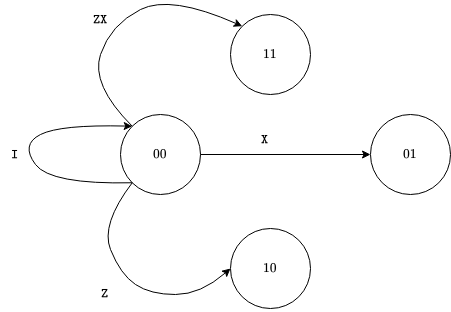
\includegraphics[width=0.65\linewidth]{body/ch5/figs/qta-fsm}
	\caption[The Quantum Finite State Machine for Emulating the Quantum Teleportation Algorithm on the FPGA.]{A quantum FSM machine which applies a switch case on the Bob's half of the EPR state base on the bit string from Alice through the quantum channel. }
	\label{fig:qta-fsm}
\end{figure}

Bob's EPR state is represented as the 32-bit output of the module in \ref{lst:qta-state-machine}. An accompanying testbench for \textit{quantum\_teleportation} module is included in listing \ref{lst:qta-tb}.
\begin{lstlisting}[language=Verilog, caption={Code snippet of the testbench for the quantum teleportation algorithm module.}, label={lst:qta-tb}]
`timescale 1ns / 1ps

module tb_quantum_teleportation;

	// Inputs
	reg clk;
	reg rst;
	reg [1:0] switches;
	
	// Outputs
	wire signed [31:0] bob_state [1:0];
	
	// Instantiate the testbench
	quantum_teleportation
	quantum_teleportation_i (
		.clk(clk),
		.rst_n(~rst),
		.switches(switches),
		.bob_state(bob_state)
	);
\end{lstlisting}
The modules are simulated in an EDA tool and synthesis in AMD Vivado. In AMD Vivado, the xdc file for the Nexys-A7 is modified to assign the inputs and controls according to hardware constraint. For this case study, the constraints that are modified corresponding to the input clock (\texttt{clk}), the active low reset (\texttt{rst\_n}) and the switches. After verification, synthesis is performed, before the final implementation is executed on the board.

The Nexys-A7 board contains various features as summarised in the table in \ref{tab:nexys-a7} below:
\begin{table}[ht!]
	\caption[Table Showing Key Features of the Nexys-A7 FPGA Board.]{Table showing the key features of the Nexys-A7 FPGA.}
	\label{tab:nexys-a7}
	\setlength\tabcolsep{0pt} % let LaTeX compute intercolumn whitespace
	\footnotesize\centering
	\begin{tabular*}{0.8\columnwidth}{@{\extracolsep{\fill}}|c|c|l|}
		\hline
		\textbf{Callout} & \textbf{Name} & \textbf{Value}\\
		\hline
		1		& PLBs  & 15850 \\
		\hline
		2		& RAM & 4860 Kbit\\
		\hline
		3		& DSPs & 240\\
		\hline
		4		& DDR2 & 128 MiB\\
		\hline
	\end{tabular*}
\end{table} 

\subsubsection{Emulating the Quantum Fourier Transform}

The high-level description of the 3-qubit QFT is shown in listing \ref{lst:qft-matlab}. The MATLAB description uses the function \texttt{tensor\_product} to perform quantum gate operations. 
\begin{lstlisting}[language=Matlab, caption={Code snippet of the MATLAB high-level description of the 3-qubit tensor product for applying quantum gate operations in the QFT quantum circuit.}, label={lst:qft-matlab}]
% ... removed code

function result = tensor_product(A, B, C)
% Tensor product of three matrices A, B, and C
	AB = zeros(size(A, 1) * size(B, 1), ...
	size(A, 2) * size(B, 2));
	for i = 1:size(A, 1)
		for j = 1:size(A, 2)
			AB((i-1)*size(B, 1)+1:i*size(B, 1), (j-1)* ...
				size(B, 2)+1:j*size(B, 2)) = A(i, j) * B;
		end
	end
	result = zeros(size(AB, 1) * size(C, 1), ...
	size(AB, 2) * size(C, 2));
		for i = 1:size(AB, 1)
			for j = 1:size(AB, 2)
				result((i-1)*size(C, 1)+1:i*size(C, 1), ...
				(j-1)*size(C, 2)+1:j*size(C, 2)) ...
			 = AB(i, j) * C;
		end
	end
end
\end{lstlisting}
Given that the system uses a 3-qubit quantum register $\ket{q_0 q_1 q_2}$ (where $\ket{q_0}$ is the LSQ), the tensor product function takes in 3 vector spaces $A$, $B$ and $C$. In cases where a single-input quantum gate is only applied to one qubit in the register, the design applies the identity gate $I$ to the remaining gate. For example, in the first time step of the QFT circuit as depicted in \ref{fig:nielsen-qft}, application of the Hadamard gate $\texttt{H}$ to the LSQ corresponds to,
\begin{align}
	\ket{q_0 q_1 q_3} = \ket{000} & = \texttt{H}\ket{0}\otimes \texttt{I}\ket{0} \otimes \texttt{I} \ket{0}\nonumber
\end{align} 
The controlled phase shift gate for 3-qubits is described by the \texttt{controlled\_phase\_shift(target, R)} MATLAB function in \ref{lst:qft-matlab-phase} which takes in the \textit{target} and \textit{R} as the inputs. The \textit{target} parameter corresponds to the the target qubit and \textit{R} represents the unitary matrix of the phase shift transformation with phase $\pi/2$.
\begin{lstlisting}[language=Matlab, caption={MATLAB code snippet for controlled phase shift quantum gates.}, label={lst:qft-matlab-phase}]
% ... removed code
	
function controlled_matrix = controlled_phase_shift(target, R)
    % Controlled phase shift gate for 3 qubits
    % Parameters:
    % - target: Target qubit (2 or 3) for applying the phase shift
    % - R: The phase shift matrix

    I = eye(2);  % Identity matrix for qubits not involved
    controlled_matrix = complex(zeros(8, 8));  
    % Initialises as complex matrix
 
    % Apply controlled phase shift gate 
    % depending on the target qubit
    if target == 2
        controlled_matrix = tensor_product([1 0; 0 1], I, I) ... 
        + tensor_product([0 0; 0 0], R, I);
    elseif target == 3
        controlled_matrix = tensor_product([1 0; 0 1], I, I) ...
        + tensor_product([0 0; 0 0], I, R);
    else
        controlled_matrix = tensor_product([1 0; 0 1], I, I) ...
        + tensor_product([0 0; 0 0], R, I);
    end
end
\end{lstlisting}
In the second time step of the QFT circuit, the controlled-$\texttt{R}_{\pi/2}$ gate is applied to the first and second qubits, with the second qubit in the register as the control and the first qubit as the target. In this case, the input phase shift gate is described in MATLAB as shown in listing \ref{lst:qft-matlab-R2}.
\begin{lstlisting}[language=Matlab, caption={MATLAB code snippet for controlled phase shift quantum gates.}, label={lst:qft-matlab-R2}]
% Controlled phase shift R2
R2 = [1, 0; 0, 2.71828^(1i * pi / 2)];  
\end{lstlisting}
Note that the natural exponent is expressed as a floating-point number ($2.71828$) since the MATLAB \texttt{exp} function does not conform to HDL Coder standards. The controlled-\texttt{T} gate with $\ket{q_2}$ as the control bit and $\ket{q_0}$ as the target, and the controlled-$\texttt{R}_{\pi/4}$ gate with $\ket{q_2}$ as the control bit and $\ket{q_1}$ as the target are also applied using the \texttt{controlled\_phase\_shift} MATLAB function. The \texttt{swap} gate between $\ket{q_0}$ and $\ket{q_2}$ is described by the function in listing \ref{lst:qft-swap}. 
\begin{lstlisting}[language=Matlab, caption={MATLAB code snippet describing the SWAP gate.}, label={lst:qft-swap}]
function SWAP = swap_gate(n)
	% Swap gate for swapping qubit 1 
	% and qubit 3 in a 3-qubit system
	SWAP = eye(8);
	
	% SWAP |000> and |111>
	SWAP([1, 8], [1, 8]) = SWAP([8, 1], [8, 1]);  
	
	% SWAP |001> and |110>
	SWAP([2, 7], [2, 7]) = SWAP([7, 2], [7, 2]); 
	
	% SWAP |010> and |101> 
	SWAP([3, 6], [3, 6]) = SWAP([6, 3], [6, 3]);
	
	% SWAP |011> and |100>  
	SWAP([4, 5], [4, 5]) = SWAP([5, 4], [5, 4]); 
end 
\end{lstlisting} 
The associated testbench is also described in MATLAB as shown in listing \ref{lst:qft-testbench}. The code snippet shows the test cases for the $\ket{000}$ state which is of interest to this design. 

\begin{lstlisting}[language=Matlab, caption={Accompying high-level description of the .}, label={lst:qft-testbench}]
% Test case 1: |000> state
% |000>
initial_state_000 = [1; 0; 0; 0; 0; 0; 0; 0];
% QFT(|000>) = |000>  
expected_000 = [1; 0; 0; 0; 0; 0; 0; 0];  
run_test_case(initial_state_000, ...
expected_000, 'Test Case 1: |000>');
\end{lstlisting}
The expected output for the test in listing \ref{lst:qft-testbench} is no phase change. To verify that the output is correct, test cases where the initial state is $\ket{001}$, $\ket{010}$ and $\ket{111}$ are also performed in a similar manner. 
 
High-level descriptions are converted to SystemVerilog using HDL Coder in MATLAB. HDL Coder automatically implements a fixed-point number scheme to optimise the operation of the algorithm in hardware. The code is synthesised in AMD Vivado where the resources that are used on the FPGA are further optimised. 

\subsubsection{Emulating the Quantum Factoring Algorithm}

The high-level description of the quantum factoring algorithm is shown in listing \ref{lst:qfa-matlab}.

\begin{lstlisting}[language=Matlab, caption={Code snippet of the MATLAB high-level description of the quantum factoring algorithm for factoring $N = 4$.}, label={lst:qft-matlab}]
	function factors = shors_algorithm(N, a)
	% Shor's Algorithm for factoring N = 21 with initial guess a = 4.
	
	% Ensure a is co-prime to N
	if gcd(a, N) ~= 1
	error('a and N must be co-prime.');
	end
	
	% Step 1: Quantum Phase Estimation
	r = find_period(N, a);
	
	if mod(r, 2) ~= 0
	disp('Order r is odd, retrying with another value of a');
	factors = [];  % Shor's algorithm fails if r is odd
	return;
	end
\end{lstlisting}
Similar to the creation of the QFT algorithm, the function is converted to SystemVerilog in HDL Coder. However, the high-level description of the quantum factoring algorithm is performed classically due to the involvement of large matrix spaces that require vast computational resources for conversion to HDL.

\subsubsection{Emulating the Quantum Search Algorithm}

The high-level description of the quantum search algorithm is developed using the MATLAB script as shown in listing \ref{lst:qsa-matlab} which uses element-wise matrix multiplications to perform the full circuit. The high-level description of the quantum search algorithm follows the quantum circuit in \ref{fig:grover-quantum-circuit} in the methodology. 
\begin{lstlisting}[language=Matlab, caption={Code snippet of the MATLAB high-level description of the quantum search algorithm perform as element-wise matrix operations.}, label={lst:qsa-matlab}]
function result = quantum_search()

	% Step 1: Initialise two-qubit register 
	% to the ground state |00>
	% |00> state for a two-qubit system
	state = [1; 0; 0; 0]; 
	
	% Step 2: Apply Hadamard gates to
	% both qubits without kron
	% Define Hadamard gate
	H = (1/sqrt(2)) * [1, 1; 1, -1];
	
	% Manually compute the tensor 
	% product of H ox H for two qubits
	H2 = [
	H(1,1)*H, H(1,2)*H;
	H(2,1)*H, H(2,2)*H
	];
	
	% Apply H2 to the initial state
	state = H2 * state;
	
	% Step 3: Apply the controlled-Z gate as the oracle
	CZ = eye(4);
	CZ(4, 4) = -1; % Controlled-Z gate flips the sign of |11> state
	state = CZ * state;
	
	% Step 4: Apply Hadamard gates to both qubits
	state = H2 * state;
\end{lstlisting}
The code snippet of the quantum search algorithm shows the first four steps from the following 8 steps for performing the full quantum circuit:
\begin{enumerate}
	\item 
	Initialise the two-qubit register to the ground-state $\ket{00}$.
	\item 
	Apply the Hadamard gates to both qubits by computing the tensor product of the two gates.
	\item 
	Apply the controlled-Z gate in the oracle to flip the phase of the bits.
	\item 
	Apply the Hadamard gate to both qubits in the oracle.
	\item 
	Apply \texttt{Z} gates to both qubits to flip relative phase of each qubit.
	\item 
	Apply the controlled-Z gate	again to flip the global phase of the system.
	\item 
	Apply Hadamard gates to both qubits to change back to the computational basis.
	\item 
	Measure the qubits to obtain the classical output by finding the highest probability outcome.
\end{enumerate}
The expected outcome of the quantum search algorithm is the classical bit string '11', however, since FPGAs support numeric types, the corresponding expected decimal output is was 3.

\subsection{User Interface Specifications}

The main function of the UIS in conjunction with the QAES is to allow user to select the quantum experiment to be performed. Quantum circuit outputs corresponding to measurements of qubits are classical bits which can be represented in decimal form and return to the user. For more complex results, the UIS takes produces graphical data on a PC running AMD Vivado. 

Given that the Nexys-A7 board has multiple switches which can be configured in by matching SystemVerilog input wires to the constraints in the board xdc file, quantum experiments can be selected as shown in table \ref{tab:quantum-select}.

\begin{table}[ht!]
	\caption[Table Showing Nexys-A7 Switch Buttons for Selecting the Quantum Experiment to be Performed.]{Table showing the switch button selection required to perform a given quantum experiment (QE).}
	\label{tab:quantum-select}
	\setlength\tabcolsep{0pt} % let LaTeX compute intercolumn whitespace
	\footnotesize\centering
	\begin{tabular*}{0.50\columnwidth}{@{\extracolsep{\fill}}|c|c|}
		\hline
		\textbf{Button} & \textbf{QE} \\
		\hline
		SW3		& Quantum teleportation \\
		\hline
		SW4	& QFT \\
		\hline
		SW5	& Quantum Factoring \\
		\hline
		SW6		& Quantum Search Algorithm \\
		\hline
	\end{tabular*}
\end{table}
In each case, the qubits are initialised to the ground state corresponding to the description in the previous section. The detection window is implemented using the $\SI{100}{\mega\hertz}$ clock of the Artix-7 FPGA. Since the decoherence time is set to $\SI{340}{\milli\second}$, the required clock rate for a detection window is $2941$.

A secondary component of the UIS subsystem is the button interface on the microcontroller which gives users the ability to transmit hard-coded bit patterns representing quantum registers or Hilbert spaces of quantum states. Bit patterns and corresponding buttons are illustrated in table \ref{tab:micro-select}
\begin{table}[ht!]
	\caption[Table Showing Nexys-A7 Switch Buttons for Selecting the Quantum Experiment to be Performed.]{Table showing the switch button selection required to transmit bit sequences through the quantum channel using the STM32 microcontroller.}
	\label{tab:micro-select}
	\setlength\tabcolsep{0pt} % let LaTeX compute intercolumn whitespace
	\footnotesize\centering
	\begin{tabular*}{0.50\columnwidth}{@{\extracolsep{\fill}}|c|c|}
		\hline
		\textbf{Button} & \textbf{Sequence} \\
		\hline
		SW0		&  $(0101)_2$\\
		\hline
		SW1		&  $(11010100)_2$ \\
		\hline
		SW2		& $(11010100)_2$\\
		\hline
		SW3		& $(10010111)_2$ \\
		\hline
	\end{tabular*}
\end{table}
The button SW4 on the microcontroller is used to reset the bit pattern. In the integrated system, the  transmission button on the STM32 microcontroller must be pressed at the same time as the SW3 switch on the Nexys-A7 board to ensure that the detection window

